\chapter{Seguridad en Docker}
\label{anexo:docker}
\section{Introducción a Docker}
Docker es una tecnología de despliegue de aplicaciones usando sistemas virtualizados en imágenes. Empaqueta las dependencias de las aplicaciones usando un \enquote{\textit{dockerfile}}. Estos archivos están siempre basados en otros, sentando como base las imágenes de sistemas operativos; los más conocidos son los de Ubuntu y Alpine, un sistema operativo Linux de 5 MB. 

Las imágenes pueden obtenerse de los distintos repositorios e incluyen toda la configuración necesaria para su implementación inmediata. Las imágenes son solo las plantillas para crear los contenedores, que serán los encargados de arrancar el sistema virtualizado, aplicar la configuración y mantenerse a la espera de instrucciones.

Los contenedores funcionan de forma independiente al sistema real y su contenido es volátil, es decir, cada vez que se para y vuelve a arrancar, el contenedor tiene el mismo estado que la imagen de origen. Esta peculiaridad es una gran ventaja en seguridad: en caso del acceso de un virus informático al sistema, un reinicio del contenedor lo eliminará. Si se configura bien, un reinicio del contenedor también obtendrá la última imagen disponible, con las actualizaciones del sistema y las dependencias correctas, simplificando enormemente el mantenimiento.

Para evitar que se borren datos persistentes existen los \enquote{volúmenes}. Un volumen es una conexión de un directorio del contenedor con uno local. Cuando se inicie por primera vez o se reinicie, el contenedor consultará este directorio.

Docker también permite la creación de redes virtuales, haciendo que ciertos contenedores no tengan acceso al exterior o entre ellos.

\begin{figure}[H]
  \centering
  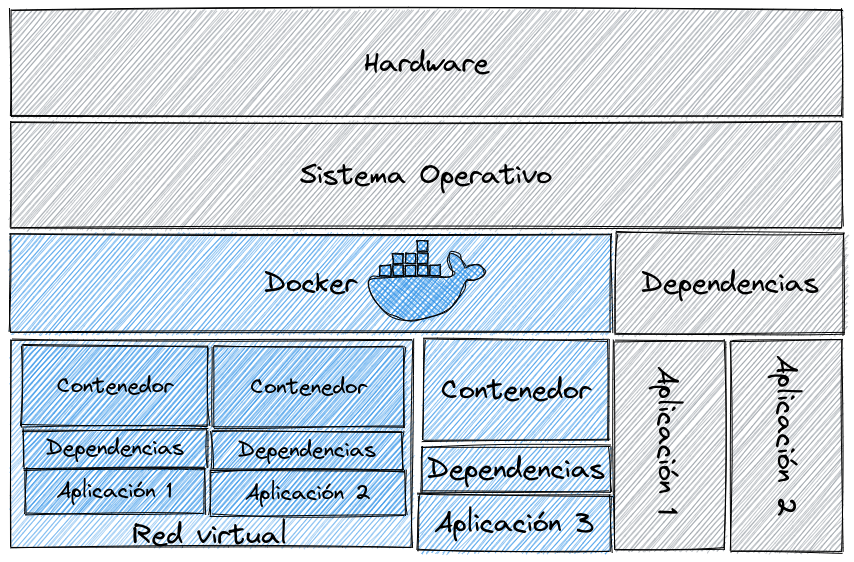
\includegraphics[width=0.5\textwidth]{docker-handraw.png}
  \caption{Funcionamiento de Docker}
  \label{fig:Docker_explicacion}
\end{figure}

\section{Docker en la seguridad}
Virtualizar aplicaciones y servicios nos permite añadir una capa más de seguridad al mantener el sistema anfitrión limpio y aislar entre los contenedores entre ellos. Una buena práctica en el uso de Docker es, por ejemplo, disponer de un contenedor MySQL para cada servicio. A la hora de montar volúmenes es posible obligar al contenedor a usar ciertos permisos y restringir la escritura. En consecuencia, el uso de contenedores nos genera las siguientes ventajas:
\begin{itemize}
    \item Los contenedores SQL se pueden incluir en una red virtual únicamente con la aplicación que las utiliza. No se podrá acceder desde otras aplicaciones ni desde \enquote{localhost}. Cada contenedor SQL dispondrá de una contraseña root distinta, una sola base de datos con un único usuario y una sola contraseña para acceso exclusivo no-root de la aplicación que lo consume.
    \item En caso de infección del contenedor y escalado de permisos, el atacante únicamente tendrá control del contenedor y, si se configura bien, no podrá escalar a un usuario del equipo anfitrión. 
    \item El puerto que se expone en el anfitrión no tiene por qué ser el mismo que el del contenedor. Si dos contenedores requieren un mismo puerto, se puede exponer uno distinto para cada uno.
    \item Los volúmenes pueden usarse para almacenar los datos de las aplicaciones en un lugar centralizado, facilitando la exportación de los datos o la creación de copias de seguridad.
\end{itemize}